% Reinforcement Learning for Dynamic Data Fragmentation and Allocation.
%
% A Deep Q-Network agent that continuously re-fragments and re-allocates
% database shards under geographically migrating workloads.
%
% COSC 6315, University of Texas Permian Basin.
%
% Build:  pdflatex main && bibtex main && pdflatex main && pdflatex main
%
% Section files live in sections/. Each one says at the top whether it is
% written or still an outline, so the state of the draft is visible without
% reading the whole thing.

\documentclass[conference]{IEEEtran}
\IEEEoverridecommandlockouts

\usepackage{cite}
\usepackage{amsmath,amssymb}
\usepackage{algorithmic}
\usepackage{graphicx}
\usepackage{textcomp}
\usepackage{booktabs}
\usepackage{tikz}
\usetikzlibrary{positioning,arrows.meta,calc}
\usepackage{url}
\usepackage[hidelinks]{hyperref}

\graphicspath{{figures/}}

\begin{document}

\title{Reinforcement Learning for Dynamic Data\\
Fragmentation and Allocation}

\author{\IEEEauthorblockN{Tinotenda Kaseke}
\IEEEauthorblockA{\textit{Department of Computer Science} \\
\textit{University of Texas Permian Basin}\\
Odessa, TX, USA \\
tinokaseke@gmail.com}}

\maketitle

\begin{abstract}
Distributed databases fix their fragmentation schema when the database is
designed and place the resulting shards with a function of the key, which
never observes where requests come from. When the geographic centre of a
workload moves, as it does daily in a multi-region service, the placement
drifts out of step with the traffic and transaction latency degrades. We
model continuous re-fragmentation and re-allocation as a Markov decision
process over a simulated six-region cluster, with a reward in which
migration cost is a fraction of the dataset rather than a byte count so
that a policy trained in simulation can be scored on real hardware without
the reward changing meaning. On a six-node CockroachDB cluster with
wide-area latency injected between nodes, gathering leaseholders in the
region issuing the transactions rather than spreading them changes p95
latency by 1372.5\,ms, which establishes the premise outside simulation.
Sweeping workload volatility over a factor of eight shows that a reactive
heuristic sits 0.44\,ms above the achievable bound under slow drift and
57.20\,ms above it under fast drift, 41\% of its own latency, whilst the
data it moves rises from 405\,GB to 1115\,GB per episode; scored under the
full objective at the highest setting it becomes indistinguishable from
static hashing. A Deep Q-Network trained at that setting beats both
baselines on held-out seeds, on two independent learner seeds, reaching a
latency 11\,ms worse than the heuristic whilst moving one twentieth of the
data. The margin is narrow, the policy had not converged, and between 80\%
and 90\% of the actions it selects are inapplicable, so the result is best
read as evidence that the room the sweep identifies is reachable rather
than as a solved problem.
\end{abstract}

\begin{IEEEkeywords}
distributed databases, data fragmentation, data allocation, reinforcement
learning, deep Q-networks, geo-distributed transactions
\end{IEEEkeywords}

% STATUS: written, 20 October 2026. Needs a figure reference in paragraph 4
% once Figure 1 exists.

\section{Introduction}

A distributed database splits its data into pieces and spreads those pieces
across machines in different places. The pieces are usually called shards, or
fragments, and the two decisions that matter are where the boundaries between
them fall and which machine holds each one. Both decisions are made once, when
the database is designed. The boundaries are fixed by a schema, and the
placement is decided by a function of the key, such as a hash, which maps a
record to a machine without ever considering where the requests for that record
come from.

That arrangement works whilst the traffic stays where the designer expected it.
In a service with users on several continents, served by a database spread
across regions in the manner of Spanner~\cite{corbett2013spanner} or
CockroachDB~\cite{taft2020cockroachdb}, it does not. The geographic
centre of the workload moves across the day as one region wakes and another
sleeps, and it moves abruptly when something local draws attention to one
region. A placement chosen for the morning is wrong by the evening. Every
request that has to cross an ocean to reach its data pays the round-trip time
of that ocean, and a transaction touching several shards held in several
regions pays it repeatedly, because the protocol that keeps such a transaction
atomic requires more than one round of agreement between the machines
involved. The result is that latency degrades steadily as the mismatch between
placement and traffic grows.

The obvious response is to move the data when the traffic moves. A simple rule
does this: each decision window, find the shard whose placement costs the most
and move it towards the region reading it. I implement that rule as a baseline
and call it \emph{follow traffic}. The question this paper asks is whether
anything is gained by replacing it with a policy learned from experience, and
the answer turns out to depend entirely on how fast the workload moves. When
drift is slow, the simple rule is within half a millisecond of the best
placement that moving shards can achieve, and there is nothing worth learning.
When drift is fast, the same rule falls 57\,ms short of that bound, which is
41\% of its own latency, because it reacts one window behind a target that has
already moved again. The room for a learned policy is therefore largest exactly
where the problem is hardest, and that is a measured observation rather than an
assumption.

This paper reports the following. I build a simulator of a six-region cluster
with a workload whose geographic centre drifts on a daily cycle and spikes
locally, and I define the placement problem on it as a Markov decision process
with a flat action space of 261 declarative actions. I establish four reference
points against which any learned policy must be judged: static hash
partitioning, which is what production systems do today; a random control; the
follow-traffic heuristic; and a per-window bound on what lease movement alone
can achieve. I measure how the gap between the heuristic and that bound widens
with workload volatility. I verify on a real six-node CockroachDB cluster, with
wide-area latency injected between the nodes, that placement changes
transaction latency by far more than the measurement noise, which is the
precondition for any of this being learnable outside simulation. Finally I
train a Deep Q-Network on the simulator and report, honestly, that it does not
yet match the heuristic, together with the evidence about why.

% TODO once Figure 1 exists: close the paragraph above with a pointer to it.

% STATUS: written, 20 October 2026.
%
% Every citation below points at a source I have read. Before submission,
% fill the entries marked VERIFY in references.bib with page numbers and
% DOIs from the publisher, and add any further related work in the three
% groups the section already sets up. Do not add a citation you have not
% opened.

\section{Related Work}

Three bodies of work meet in this problem: the classical treatment of
fragmentation and allocation as an optimization to be solved, recent systems
that adapt placement to a moving workload, and the use of learning to replace
hand-written database administration.

\subsection{Fragmentation and allocation as an optimization problem}

The question of how to divide a database and where to put the pieces is as old
as distributed databases themselves, and the classical treatment is to state it
as an optimization problem and solve it once. A cost model scores a candidate
arrangement against an expected workload, and a solver searches for the
arrangement that minimizes it. The result is then installed and the database
runs with it.

The weakness is in the word once. A solved-once answer is correct for the
workload it was solved against and degrades as the real workload departs from
it. Where the departure is slow this is tolerable, and where the workload has a
geographic centre that moves on a daily cycle it is not. That observation
motivates the systems in the next group, which re-solve the problem as the
workload changes.

% TODO: cite two or three classical treatments here. Candidates to read:
% vertical and horizontal partitioning in distributed database design, and
% the allocation problem as stated in the standard textbook treatment.

\subsection{Adapting placement to a moving workload}

Lion~\cite{lion2024} is the closest system to this work in intent. It observes
that a transaction is slow mainly because it spans machines, and it therefore
arranges replicas so that some single node holds a copy of every partition a
given transaction touches, allowing that transaction to commit locally rather
than through the multi-round agreement protocol that a distributed commit
requires. A graph-based analyzer groups partitions that are accessed together,
a cost model assigns those groups to nodes subject to a load-balance
constraint, and an LSTM predictor forecasts the workload so that replicas are
provisioned before the shift rather than after it. Lion reports up to 2.7 times
higher throughput and 76.4\% better scalability than the approaches it is
compared against.

Lion establishes three things this work depends on. Adapting placement to a
moving workload is worth a large amount of real throughput. Migration cost and
load balance both belong in the objective rather than latency alone.
Anticipating a shift beats reacting to one, by roughly a factor of four in
adaptation speed.

It also leaves three openings. The adaptation is a heuristic pipeline rather
than a learned policy: the LSTM forecasts, but a hand-written cost model
decides, so the system never improves from the outcomes of its own decisions.
Geographic distance does not appear in its cost function, which is expressed in
bytes moved, so two placements that differ by an ocean score identically.
Fragment boundaries are fixed, so Lion moves replicas of a partition but never
splits one.

GeoTP~\cite{geotp2025} supplies the geographic dimension that Lion does not
have. It targets database middleware connecting heterogeneous data sources
across regions, where the dominant costs are the network latency between the
middleware and its data sources and the length of time a transaction holds
locks whilst waiting on remote work. GeoTP reduces both: a decentralized
prepare phase cuts the number of network round trips a distributed transaction
needs, and a latency-aware scheduler delays lock acquisition so that the
contention window is shorter. It reports up to 17.7 times improvement on YCSB
and TPC-C.

GeoTP shows that latency awareness is worth building a scheduler around, and
its cost accounting is the model for the one used here. It optimizes the
execution of transactions against a given placement, however, and does not
change where the data sits. The two papers are therefore complementary, and
the gap between them is where this work sits: Lion adapts placement without
seeing geography, GeoTP sees geography without adapting placement.

\subsection{Learning to administer a database}

A separate line of work replaces hand-written database administration with
learned policies, in index selection, in configuration tuning, and in query
optimization. The common argument is that these decisions are made repeatedly
against a changing workload, that the quality of a decision is measurable after
the fact, and that a system able to learn from its own outcomes should
eventually beat a fixed rule written by a person who could not anticipate every
workload.

Placement is a natural member of that family and has received less attention
than the others, which is the opportunity this work takes up.

% TODO: cite representative learned index selection, knob tuning and query
% optimization work. Read at least one from each before citing it.

\subsection{What is new here}

This work learns fragmentation and geographic placement \emph{jointly}, as one
policy, for transactional workloads. Lion learns neither and adapts only
replica placement. GeoTP optimizes execution rather than placement. The learned
administration literature addresses other decisions. Stating the contribution
precisely: the agent chooses, in one action space, where a shard's primary copy
sits, where its replicas sit, and where the boundary between two shards falls,
and it is rewarded on a cost that combines transaction latency, the volume of
data moved, and load imbalance.

I state one limitation of the contribution up front, because the evaluation
reports it. The agent described here is wired, trained and measured, and it
does not yet outperform the hand-written heuristic it is meant to replace.
What this paper establishes is the problem, the measurement apparatus, the
baselines, and the conditions under which a learned policy has room to win.

% STATUS: written, 20 October 2026.
%
% Most of this is transcribed from docs/mdp-specification.md and
% docs/adr/ADR-0002-flat-declarative-action-space.md. If either of those
% changes, change this with it.

\section{System Model and Methodology}

\subsection{What is being decided}

A cluster has $R$ regions, each holding one database node. The keyspace is
divided into $C$ atomic cells, and a \emph{shard} is a contiguous run of cells.
Each shard has one \emph{primary} copy, which serves writes, and some number of
\emph{replicas}, which hold the same data and can serve reads. The number of
replicas per shard, called the replication factor, is fixed at three throughout
this work and is not something the agent controls.

Three decisions are therefore available at any moment. Which region holds a
given shard's primary. Which regions hold its replicas. Where the boundary
between two shards falls. The first two are allocation and the third is
fragmentation, and this work treats them as one problem because they interact:
splitting a shard is only worth doing if the two halves are then placed
differently.

\subsection{The cost of a placement}

Latency is computed analytically from a fixed matrix of round-trip times
between regions. A read costs the round trip to its nearest copy. A write costs
the round trip to the primary plus the time for a majority of replicas to
acknowledge it, since a write is not durable until enough copies agree. A
transaction touching several shards costs its member operations plus, if those
shards' primaries sit in more than one region, an additional charge for the
two-phase commit protocol that keeps it atomic.

That last term is the mechanism this work is built on. It is what makes placing
together two shards that are used together worth something, and therefore what
makes the fragmentation decision interact with the allocation decision.

\subsection{The workload}

The workload generator produces a stream of requests whose geographic origin
moves. Each of the $C$ cells sits at an angular position on a circle, as do the
regions, and traffic for a cell originates predominantly from whichever regions
sit near its angle. The whole angular field rotates over a daily period, which
is what makes a placement chosen at one time wrong at a later one. Cell
popularity follows a Zipf distribution, so a minority of cells carry most of
the traffic, and localized spikes arrive as a Poisson process, multiplying one
region's traffic for a short burst. The read and write mix and the skew
parameter follow the YCSB conventions~\cite{cooper2010ycsb}, so the workload is
recognizable rather than invented, with geographic origin added as the dimension
YCSB does not model.

Adjacent cells are given correlated but not identical angular positions by a
random walk. This is the detail that makes splitting worthwhile: a wide shard
spans divergent angles and therefore cannot be placed well anywhere, whilst its
two halves can each be placed well.

A single parameter, \emph{volatility}, scales the rotation speed, the spike
rate and the spike size together, so one number moves the environment from
placid to violent. It is the main axis the evaluation sweeps.

\subsection{The decision problem}

The problem is stated as a Markov decision process. The agent acts once per
decision window.

\paragraph{Observation} The state is encoded as a fixed-length vector
describing, for every shard, its size and the regions holding its primary and
replicas; for every region, its share of requests and its storage occupancy;
the recent history of data movement; the matrix of inter-region round-trip
times; and a small set of scalars summarizing current cost.

\paragraph{Actions} The action space is flat and declarative, with 261 actions
at $R=6$ regions and a cap of 20 shards. Four kinds:

\begin{itemize}
\item \textsc{move\_lease}$(f, r)$ makes region $r$ the primary for shard $f$.
It moves no data and is only legal where $r$ already holds a replica.
\item \textsc{move\_replica\_to}$(f, r)$ places a replica of shard $f$ in
region $r$, evicting the existing replica furthest from $r$ so that the
replication factor stays constant. It costs one shard's worth of movement.
\item \textsc{split}$(f)$ divides shard $f$ at its midpoint.
\item \textsc{noop} does nothing.
\end{itemize}

Two properties of this encoding matter. First, every action names a desired end
state rather than an operation, so every action is defined in every state: an
action that cannot be applied resolves to a small penalty rather than an
error. This matters because a Deep Q-Network cannot mask illegal actions, so an
action space with illegal members would need machinery that this one avoids.
Second, the encoding was chosen by measurement rather than by taste. The
destination-only form of \textsc{move\_replica\_to} gives 261 actions against
861 for the naive source-and-destination form, with a higher fraction of
actions applicable in a typical state, and a breadth-first search over the
reachability graph confirms that no placement becomes unreachable.

\paragraph{Reward} The reward is the negative weighted sum of three normalized
terms: mean latency divided by a scale constant, data moved as a fraction of
the total dataset, and load imbalance. Expressing movement as a fraction of the
dataset rather than in bytes is deliberate and necessary: the simulator holds
60\,GB and the real cluster used for validation holds about 1\,GB, and a reward
denominated in bytes would score the same physical move sixty times
differently in the two environments, making a policy pre-trained in one
meaningless in the other.

\subsection{Baselines}

Four reference points. Three are policies and one is a bound.

\begin{itemize}
\item \textbf{Static hash} never moves anything. The initial placement is what
a consistent-hash partitioner~\cite{karger1997consistent} produces, and it is
held for the whole episode.
This is what a production database does today and it is the thing to beat.
\item \textbf{Random} selects a legal action uniformly. It is a control: it
proves that any gain comes from choosing \emph{where} to move data rather than
from moving data at all.
\item \textbf{Follow traffic} finds, each window, the single shard whose
primary placement costs the most relative to the best available region, and
moves it towards that region. It is the obvious rule an operator would write by
hand, and it is myopic by construction, weighing no migration cost and
anticipating no drift.
\item \textbf{Best per window (fixed shards)} is not a policy. It is the lowest
latency reachable by relocating every primary for free and instantly, each
window, at the shard boundaries the episode started with. No real policy can
reach it, because it pays no movement cost and sees the window it is
optimizing. It is also not a global optimum, because it never splits a shard, so
a policy that splits can legitimately sit below it.
\end{itemize}

\subsection{The agent}

The agent is a Deep Q-Network. A Q-network is a function that, given the
current state, estimates the long-run value of each available action; the
policy is then to take the action with the highest estimate. The network here
has two hidden layers of 256 units and is trained with the standard
Stable-Baselines3 implementation~\cite{raffin2021sb3} against a Gymnasium
environment~\cite{towers2025gymnasium}, following Mnih et
al.~\cite{mnih2015dqn}.

The plain form is used deliberately, without the extensions that
Rainbow~\cite{hessel2018rainbow} combines: double Q-learning to correct
overestimation~\cite{vanhasselt2016double}, a dueling
head~\cite{wang2016dueling}, or prioritized replay~\cite{schaul2016per}. The
question here is whether the problem is learnable at all, and establishing that
with the simplest agent makes any later improvement attributable to the
extension rather than to the combination. The evaluation reports where that
choice costs something.

Two choices in the training setup are worth stating because they are easy to
get wrong. Training resets onto a rotating set of 64 workload seeds rather than
one, because an agent trained on a single realization learns that realization
rather than the structure behind it. Evaluation uses a block of seeds disjoint
from the training seeds and acts greedily rather than exploring, so the
reported number is generalization rather than recall.

\subsection{Metrics}

Every result in this paper reports some subset of five quantities.

\begin{itemize}
\item \textbf{Mean latency}, in milliseconds, averaged over the windows of an
episode.
\item \textbf{p95 latency}, the value below which 95\% of observations fall. It
is reported alongside the mean because an average can hide a bad tail, and
users experience the tail.
\item \textbf{Data moved}, in gigabytes per episode. This is the price paid for
whatever latency was bought.
\item \textbf{Cross-region transaction fraction}, the share of transactions
whose shards span more than one region and which therefore pay the two-phase
commit charge.
\item \textbf{Load imbalance}, a measure of how unevenly requests are spread
across regions, included because a policy can lower latency by piling all the
work onto one region, which is not a real improvement.
\end{itemize}

Results are reported as the mean over eight seeds with a 95\% percentile
bootstrap~\cite{efron1979bootstrap} confidence interval computed over those
seeds. The bootstrap is used rather than a $t$ interval because eight is a small
sample and nothing guarantees the per-seed means are normally distributed.

\subsection{Experimental apparatus}

Every number reported here comes from a single script that writes one
self-contained directory per run, holding the resolved configuration, the seed
list, the commit the code was at, the package versions, the machine, the raw
per-window record, the per-seed summary, and the exact command that reproduces
the run. Runs execute on GitHub Actions rather than on a personal machine, so
each is unattended and each records the hardware it received. This is reported
because it is part of the method: a number that cannot be traced to the
configuration that produced it cannot be defended.

\subsection{Validation on a real cluster}

The structure of pre-training in a cheap simulator and fine-tuning on expensive
real hardware is borrowed from robotics, where it is standard and where the gap
between the two is the central difficulty~\cite{tobin2017domain}. The difference
here is that the gap is narrower and more checkable: the simulator and the
cluster can be made to agree on the observation space, the action space and the
cost structure by construction, which is why the database was chosen for that
property.

The simulator's cost model is an assumption, and the assumption is testable.
I deploy six CockroachDB~\cite{taft2020cockroachdb} nodes, one per simulated
region, in containers on a single host, with wide-area round-trip times injected
between them using the Linux kernel's traffic control facility. CockroachDB was
selected over sixteen other candidate systems on one criterion: it exposes a \emph{synchronous}
statement for relocating a shard's lease and its replicas. Synchrony is
essential rather than convenient. If a placement command returns before the
placement has changed, the reward observed after an action belongs to a state
the action did not produce, and the decision problem is no longer well defined.

\begin{figure}[t]
\centering
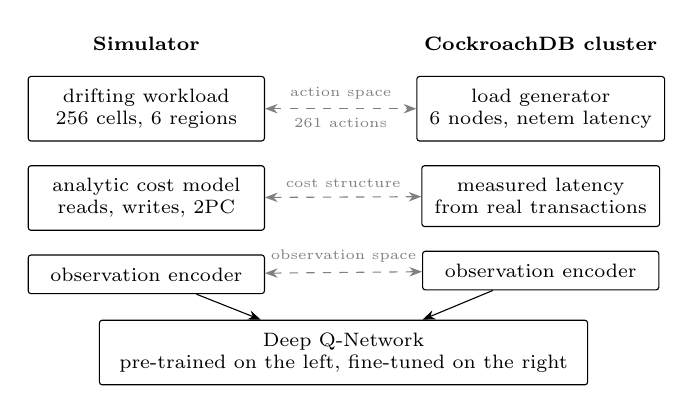
\begin{tikzpicture}[
  node distance=3mm,
  box/.style={draw, rounded corners=1pt, align=center, font=\scriptsize,
              minimum width=30mm, inner sep=1.6mm},
  title/.style={font=\scriptsize\bfseries},
  parity/.style={<->, >={Stealth[length=1.6mm]}, dashed, gray},
  note/.style={font=\tiny, gray, align=center}
]

% Left column: the simulator.
\node[title] (simtitle) {Simulator};
\node[box, below=2mm of simtitle] (simwork) {drifting workload\\256 cells, 6 regions};
\node[box, below=of simwork] (simcost) {analytic cost model\\reads, writes, 2PC};
\node[box, below=of simcost] (simobs) {observation encoder};

% Right column: the real cluster.
\node[title, right=26mm of simtitle] (clutitle) {CockroachDB cluster};
\node[box, below=2mm of clutitle] (cluwork) {load generator\\6 nodes, netem latency};
\node[box, below=of cluwork] (clucost) {measured latency\\from real transactions};
\node[box, below=of clucost] (cluobs) {observation encoder};

% The three parity constraints.
\draw[parity] (simwork) -- node[note, above] {action space} node[note, below] {261 actions} (cluwork);
\draw[parity] (simcost) -- node[note, above] {cost structure} (clucost);
\draw[parity] (simobs) -- node[note, above] {observation space} (cluobs);

% The agent, underneath, moving left to right.
\node[box, below=6mm of $(simobs)!0.5!(cluobs)$, minimum width=62mm]
  (agent) {Deep Q-Network\\pre-trained on the left, fine-tuned on the right};
\draw[->, >={Stealth[length=1.6mm]}] (simobs) -- (agent);
\draw[->, >={Stealth[length=1.6mm]}] (cluobs) -- (agent);

\end{tikzpicture}
\caption{The two halves of the system and the three things that must agree
between them. The agent is pre-trained against the simulator, which is fast and
cheap, and fine-tuned against the cluster, which is slow and real. Transfer is
only meaningful if the observation space, the action space and the cost
structure are the same on both sides, which is why the database was chosen for
its ability to satisfy them rather than for its popularity.}
\label{fig:architecture}
\end{figure}

% STATUS: OUTLINE ONLY. The rubric awards zero points for this section at
% the midterm, so it exists to show the structure. Every number below is
% already measured and recorded; what is missing is the prose and the
% figures, which is Thursday and Friday's work.
%
% Every figure listed here has a run directory behind it. Take the number
% from the run directory, never from this file, and never from memory.

\section{Evaluation}

% ---------------------------------------------------------------------
\subsection{Questions}
% Four, in order:
%   Q1  Does placement matter at all on a real cluster?
%   Q2  How much does following the traffic beat doing nothing?
%   Q3  How does that advantage change as the workload moves faster?
%   Q4  Does a learned policy beat the heuristic?
% Q4's answer is "not yet", and the section is structured so that is
% reported rather than buried.

% ---------------------------------------------------------------------
\subsection{Setup}
% Six regions, replication factor 3, 256 cells, 200 decision windows per
% episode, eight seeds. Round-trip matrix stated as a table.
% Cluster: six CockroachDB nodes in containers, netem latency injection
% accurate to 0.1 ms across the measured pairs.
% Hardware: GitHub Actions ubuntu-latest, 2 cores, 7 GB. State this.

% ---------------------------------------------------------------------
\subsection{Q1: placement changes latency on a real cluster}
% Source: Cluster pilot #2, 20 October 2026, docs/results-log.md run 2.
%
%                        p50      p95      stdev
%   leases co-located    272.7    275.5    48.8
%   leases spread       1013.4   1648.0   302.0
%   p95 gap 1372.5 ms
%
% THREE THINGS THAT MUST APPEAR IN THIS SUBSECTION:
%
% 1. "Co-located" means the leases, not the data. With replication factor
%    3 and one node per region, three replicas cannot fit in one region,
%    so every write pays a cross-region quorum even in the co-located
%    case. That is why the co-located p50 is 272.7 ms and not single
%    digits. The experiment isolates the leaseholder effect, which is
%    exactly what MOVE_LEASE corresponds to.
% 2. The confidence interval is indicative, not a precision claim. At
%    N = 200 transactions the p95 is the 190th order statistic, so the
%    bootstrap interval is degenerate at the top. Report the gap, report
%    N, say the interval is indicative, and state that choosing N by
%    measurement is outstanding work.
% 3. Six database processes shared two cores. Say so.

% ---------------------------------------------------------------------
\subsection{Q2: following the traffic beats doing nothing}
% Source: Experiments #1, 20 October 2026, 8 seeds, volatility 1.0.
%
%   Static hash                      156.11  [148.92, 164.33]     0.0 GB
%   Random                           158.02  [150.98, 165.63]   204.8 GB
%   Follow traffic                    98.66  [ 89.49, 106.58]   785.2 GB
%   Best per window (fixed shards)    93.66  [ 86.60,  99.63]     0.0 GB
%
% 36.8% improvement. Note that random is no better than static despite
% moving 205 GB, which is the point of including it: the gain comes from
% choosing where, not from moving.
%
% TABLE 1 goes here.

% ---------------------------------------------------------------------
\subsection{Q3: the advantage collapses as the workload moves faster}
% Source: Sweep #1, 20 October 2026, 8 seeds per value.
% THIS IS THE SECTION THE PAPER IS FOR. Give it the space.
%
%   volatility   static   follow   bound    headroom   advantage
%        0.5     156.27    94.31   93.87     0.44 ms      39.7%
%        1.0     156.11    98.66   93.66     5.00 ms      36.8%
%        2.0     155.37   125.37   89.47    35.90 ms      19.3%
%        4.0     155.77   139.58   82.38    57.20 ms      10.4%
%
%   GB moved by follow traffic: 405 -> 785 -> 1057 -> 1115
%
% The three observations, in this order:
%
%   (a) Static hashing is flat. It does not degrade with volatility
%       because it was never tracking anything. Say this plainly; it is
%       the reason the advantage column falls rather than the baseline
%       rising.
%   (b) The bound IMPROVES with volatility, 93.87 -> 82.38, because
%       sharper traffic concentration means a well-chosen placement does
%       better. So the achievable optimum gets better whilst the
%       heuristic gets worse. That widening gap is the finding.
%   (c) The heuristic pays more and gets less: movement rises from
%       405 GB to 1115 GB whilst its advantage falls from 39.7% to
%       10.4%. A reactive rule under fast drift is buying churn.
%
% The conclusion to draw: the room for a learned policy is largest
% exactly where the problem is hardest. At volatility 0.5 there is
% nothing to win. At volatility 4 there is 41% of the heuristic's own
% latency to win.
%
% FIGURE 2 goes here, two panels: latency against volatility, and GB
% moved against volatility. Source: results/sweeps/volatility/sweep.png.

% ---------------------------------------------------------------------
\subsection{Q4: the learned policy does not yet match the heuristic}
% Sources: Train agent #1 and #2, 20 October 2026, both at volatility 1.0,
% both evaluated on held-out seeds 2000-2007.
%
%   run 1, w_migration = 0.30:   146.55 ms,  53.2 GB moved
%   run 2, w_migration = 0.00:   135.57 ms, 192.8 GB moved
%   follow traffic:               90.76 ms, 752.6 GB moved
%
% Report this straight. The structure of the argument:
%
%   (a) Run 1 learned to sit still: 53 GB against the heuristic's 753.
%       The migration penalty is immediate and certain whilst the latency
%       benefit is delayed and spread over later windows, and a Q-function
%       trained for 1,500 episodes resolves that disagreement by not
%       moving.
%   (b) Run 2 removed the penalty entirely. Movement rose to 193 GB and
%       latency improved by 11 ms, which confirms (a) as a contributing
%       cause but does not close the gap.
%   (c) Run 2's held-out evaluation was still improving at the final
%       training step, 127.66 ms at step 300,000 against run 1's plateau
%       at 138 ms by step 160,000. The budget ran out before convergence.
%   (d) Both runs trained at volatility 1.0, where the sweep shows the
%       available headroom is 5 ms. The agent was asked to win a contest
%       with almost no prize. Training at volatility 2 to 4 is the
%       obvious next experiment and is outstanding work.
%
% FIGURE 3: training curve, held-out latency against timestep, both runs.
% Source: eval_history.json in each model directory.

% ---------------------------------------------------------------------
\subsection{Threats to validity}
% - The simulator's cost model is analytic. Q1 validates that placement
%   matters on real hardware; it does not validate the magnitudes.
% - Two cores for six database processes adds scheduling noise.
% - N = 200 transactions was chosen by convenience rather than by
%   measurement.
% - The bound holds the starting shard boundaries, so it is not a global
%   optimum and should not be read as one.
% - The agent selects inapplicable actions in 80-90% of windows. Cite
%   \cite{huang2022masking} for why masking matters as the invalid share
%   grows, and \cite{zahavy2018elimination} for an action-elimination
%   network built on DQN specifically, which is the closest published fix.
% - Results at volatility 1.0 should not be generalized to other
%   volatilities, which is precisely what Q3 demonstrates.

% STATUS: OUTLINE ONLY. Zero points at the midterm. Write it after the
% Evaluation section, because a conclusion written first tends to describe
% the result you hoped for.

\section{Conclusion and Future Work}

% ---------------------------------------------------------------------
% WHAT TO SAY, in about three paragraphs.
%
% 1. What was established. The problem stated as an MDP with a measured
%    action encoding; four baselines; a validated cost assumption on real
%    hardware; and the measured relationship between workload volatility
%    and the room available to a smarter policy.
%
% 2. The main finding. A reactive heuristic is near-optimal under slow
%    drift and falls 41% short of the achievable bound under fast drift,
%    whilst moving nearly three times as much data. The case for learning
%    is therefore conditional on volatility, and that condition is now
%    measured rather than assumed.
%
% 3. What was not achieved. The agent does not yet beat the heuristic.
%    Say it in one sentence, without hedging, and then say what the
%    evidence points at.

% ---------------------------------------------------------------------
\subsection{Future work}
% In the order they should be attempted:
%
% 1. Train at volatility 2 to 4, where there is something to win.
% 2. Address credit assignment: n-step returns, or reward shaping that
%    credits a move with the latency it saves in later windows rather
%    than charging it entirely at the moment it is made.
% 3. Longer training. Run 2 had not converged at 300,000 steps.
% 4. Fine-tune the pre-trained agent on the real cluster. The apparatus
%    exists and the parity constraints are satisfied; the harness is not
%    yet built.
% 5. Choose N by measurement and re-run the cluster experiment.
% 6. Add a cost-model rebalancer in the style of Lion as a stronger
%    baseline than follow traffic.


\bibliographystyle{IEEEtran}
\bibliography{references}

\end{document}
